\section{CMS}
CMS ofrece un ambiente orientado a objeto para diseñar aplicaciones de usuario. CMS ofrece a la aplicación la posibilidad de modelar su comportamiento en la forma de objeto. Este elemento de servicio ofrece variables, eventos que se utilizan para diseñar y especificar como la funcionalidad de un módulo puede acceder a las interfaces CAN.

El servicio asume que no hay fallas provenientes de la capa de enlace de datos y la capa física de la red CAN. Las fallas, si ocurren, son resueltas por el NMSE (Network Management Service Element).

\subsection{Prioridades de los objetos}
La arbitración del protocolo CAN se realiza teniendo en cuenta la prioridad de los identificadores de los frames que se envía. La arbitración es no destructiva, debido a la necesidad de de tener un procesamiento de mensajes de tiempo real. La prioridad se determina teniendo en cuenta cada uno de los bits. El indentificador de los objetos y eventos de CMS está compuesto por 8 bits más 3 bits que los diferenciará entre objetos y eventos. Los eventos tiene mayor prioridad.

\begin{tabular}{lll}
    000 & (ID) & Tipo de evento \\
    111 & (ID) & Prioridad objeto \\
\end{tabular}

La prioridad de los objetos es un UInteger de 1 byte. La prioridad más baja es 0 y la prioridad más alta de 1. Por lo tanto la prioridad va desde 00000000b (mayor prioridad) hasta 11111111b (menor prioridad).

\subsection{Objeto CMS}
Un objeto CMS define una estructura de dato que se debe respetar para poder enviar información (variables) a través de la red. El objeto está compuesto por los siguientes campos:
\begin{itemize}
   \item Name: string de 6 caracteres (6 bytes)
   \item User\_type: {client, server} (1 bit)
   \item Priority: UInteger (1 bytes)
   \item Datatype: UInteger identificador del tipo de datos (1 byte)
   \item Data: Indefinido.
\end{itemize}

\begin{figure}[h!]
 \centering
 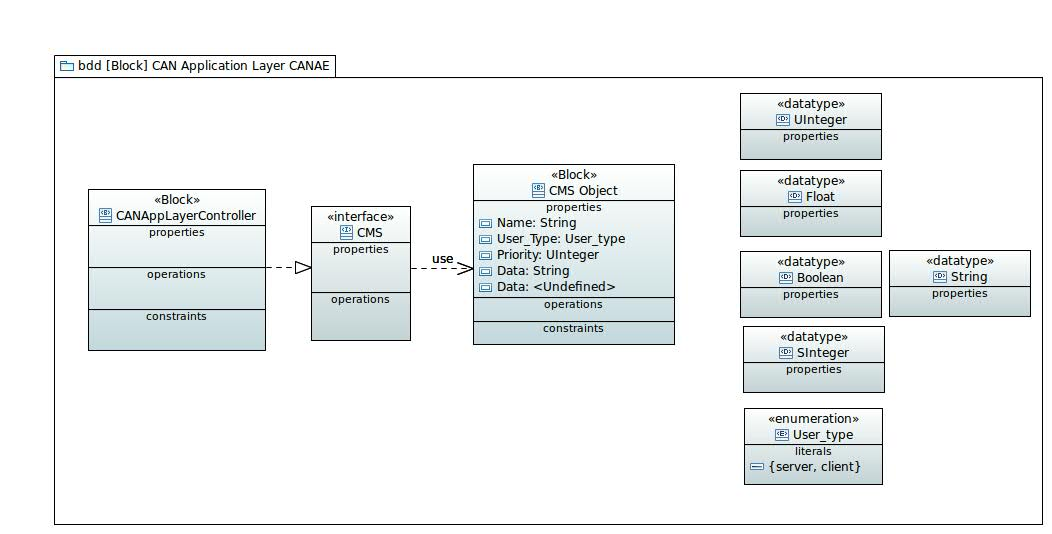
\includegraphics[scale=0.4]{images/Secciones/AppendixA/CMSObject.JPG}
  \caption{Definición del Objeto CMS}
\label{fig:CMSObject}
\end{figure} 

\subsection{Servicios de CMS}
Con respecto a las variables de CMS existen una serie de servicios brindados por CMS, que pueden ser tanto \textit{local services} como \textit{remote services}. Su clasificación depende de si se está accediendo a variables almacenadas dentro del nodo, o bien se está intentando acceder (escribir o leer) una variable remota. Un evento está definido de la siguiente manera:

\begin{itemize}
   \item Name: string de 6 caracteres (6 bytes)
   \item User\_type: {client, server} (1 bit)
   \item Priority: UInteger (1 bytes)
   \item Event\_Type: UInteger identificador del tipo de datos (1 byte)
   \item Data: Indefinido.
\end{itemize}


\subsubsection{Servicios locales}
\begin{itemize}
  
\item Boolean define\_variable(String name, DataType data\_type)
  \begin{itemize}
  \item \textbf{String name}: Nombre de la variable.
    \item \textbf{DataType data\_type}: Tipo de dato de la variable. 
  \end{itemize}
  
\item Boolean set\_variable(String name, UInteger destination, Data data, UInteger priority)
  \begin{itemize}
    \item \textbf{String name}: Nombre de la variable.  
    \item \textbf{UInteger destination}: Direción del destinatario. Esta dirección debe ser provista por el NMT.
    \item \textbf{Data data}: Datos a enviar.
    \item \textbf{UInteger priority}: Prioridad de la variable.
  \end{itemize}
  
\item Boolean update\_variable(String name, data data)
  \begin{itemize}
    \item \textbf{String name}: Nombre de la variable
    \item \textbf{Data data}: Datos a enviar    
  \end{itemize}
 
\end{itemize}
\subsubsection{Servicios remotos}
\begin{itemize}
\item Boolean write\_variable(String name, Data data)
  \begin{itemize}
    \item \textbf{String name}: Nombre de la variable a escribir
    \item \textbf{Data data}: Dato a escribir
  \end{itemize}
\item Data read\_variable(String name)
  \begin{itemize}
    \item \textbf{String name}: Nombre de la variable a leer
  \end{itemize}
\end{itemize}

\subsection{Eventos}
Los eventos se utilizan para modelar comportamientos asíncronos, tales como temperatura excedida en un tiempo determinado. La ocurrencia de los eventos es detectada por el nodo, que en ese momento actuará como server y se notifica a todos los clientes.
\begin{comment}
\begin{figure}[h!]
 \centering
 \includegraphics[scale=0.4]{images/Secciones/AppendixA/CMSEvent.JPG}
  \caption{Definición del Objeto CMS}
\label{fig:CMSEvent}
\end{figure} 
\end{comment}
Los servicios al igual que las variables se dividen los eventos brindados por servicio local o servicio remoto. Los servicios se describen a continuación.

\subsubsection{Servicios locales}
\begin{itemize}
\item define\_event(String name, UInteger priority, UInteger event\_type)
  \begin{itemize}
  \item \textbf{String name}: Nombre del evento
  \item \textbf{UInteger priority}: Prioridad del evento
  \item \textbf{UInteger event\_type}: Tipo de evento según tabla \ref{table:prioridad_eventos}
  \end{itemize}

\end{itemize}

\subsubsection{Setvicios remotos}

\begin{itemize}
\item Event notify\_event()
\item Boolean store\_event(String name)
  \begin{itemize}
    \item \textbf{String name}: Nombre de evento a almacenar
  \end{itemize}
  
\item Event read\_event(String name)
  \begin{itemize}
    \item \textbf{String name}: Nombre de la variable a leer
  \end{itemize}
\end{itemize}

\subsubsection{Prioridad de eventos}
La prioridad de los eventos se define como una tabla que se define al momento de implementar el protocolo. Al desarrollar la tabla de prioridades se debe cuidar la relevancia de los eventos. La prioridad más baja es 0. El tamaño de la prioridad del evento es de 1 byte. Por lo tanto la prioridad va desde 00000000b (mayor prioridad) hasta 11111111b (menor prioridad).

\begin{table}[h!]
  \centering
  \caption{Prioridad eventos}
  \label{table:prioridad_eventos}
  \begin{tabular}{|l|l|l}
    \cline{1-2}
    00000000 & Nombre evento & Mayor prioridad \\\cline{1-2}
    00000001 & Nombre evento & \\\cline{1-2}
    00000010 & Nombre eevnto & \\\cline{1-2}
    ... & ... & ... \\\cline{1-2}
    11111111 & Nombre evento & Menor prioridad \\\cline{1-2}
  \end{tabular}    
\end{table}

Esta tabla de prioridad de eventos, debe ir acompañada de un diccionario de eventos, donde se almacena los datos relevantes al evento. En esta se hace una descripción del evento. Sirve de guía para la implementación y desarrollo de aplicaciones que identifican eventos.

El diccionario debería incluir los siguientes campos:
\begin{itemize}
\item Nombre del evento
\item Descripción del evento
\item Prioridad
\item Umbral límite inferior (En el caso de que existiera)
\item Umbral límite superior (En el caso de que existiera)
\end{itemize}



